\documentclass[10pt,twocolumn,letterpaper]{article}
\usepackage[margin=0.75in,columnsep=0.25in]{geometry}
\usepackage[T1]{fontenc}
\usepackage{newtxtext,newtxmath,graphicx,booktabs,longtable,microtype}
\usepackage[hidelinks]{hyperref}
\setlength{\parindent}{1em}
\raggedbottom
\begin{document}
\setcounter{section}{6}\setcounter{subsection}{4}
\subsection{Filesystem Reuse in Applications}
\label{sec:filesystem-reuse}

Container image access puts the same filesystem format in two execution
environments: the native kernel serves mounted filesystems, while a user
reader serves container images. SquashFUSE implements the latter directly;
LKL and Rump instead bring kernel filesystem implementations into user
environments~\cite{ev_squashfuse062,ev_lkl_source,kantee2009rump}.
We test whether VKSO can use one resident native execution body for both
purposes, with independent objects and practical application costs.
Native SquashFS and real Apptainer SIF execution provide the case study.
SquashFUSE and LKL are executable application baselines; an identical-code
copied backend isolates VKSO's additional physical-sharing property.

\paragraph{What is reused.}
The prepared Linux~5.15.198 filesystem places 34 functions, containing
2,103 original physical source lines, in a common owner. They implement
superblock, inode, directory, block-list, metadata and data-access logic.
The native consumer retains VFS objects, synchronization and BIO services.
The user bridge supplies its own objects, caches and POSIX input through
46 filesystem service bindings; ten further fields hold native operation
tables and are null in the FUSE bridge.

The final owner also contains the safe LZ4 decoder from Section~6.3 and the
matching kernel's XZ stream, LZMA2 and BCJ decoder bodies. The three XZ
algorithm files retain all 2,604 original physical lines without body edits;
nine private allocation, memory and CRC services supply their environment.
LZ4 uses three private memory-service slots. Native XZ retains its PREALLOC
mode, while the user interface supplies complete contiguous blocks in SINGLE
mode. Both user backends remove their liblz4 and liblzma dependencies.
Thus composition extends the executed reuse boundary beyond filesystem
parsing, while leaving gzip, zstd and lzo decoding as domain-specific services.
The owner's executable text grows from 16,695 to 27,828 bytes relative to the
preceding LZ4-composed version; physical sharing is measured separately below.

A single-threaded, read-only FUSE frontend connects the bridge to
Apptainer~1.5.5~\cite{ev_apptainer155}. A 96-line C translator accepts the
application's helper arguments, including its open file descriptor and SIF
partition offset. Apptainer and the container programs retain their sources.
The user environment keeps inode and name objects until unmount.

\paragraph{Functional and physical evidence.}
Original native, prepared native before/after sharing, copied and shared
readers pass 25 five-format mounts with content, metadata, links, extended
attributes and boundary checks. Each user backend additionally passes
22,032 boundary/random-offset reads over six cases. A separate x86 BCJ
fixture verifies the selected filter chain and both-domain reads.
The interface exposes read-only operations and user/security attributes.

The final owner shares seven code and two readonly pages (36~KiB) with
the kernel; copied execution uses identical mapped bytes on different PFNs.
The filesystem and codec bindings have private backing and user-space
targets. Native xz and lz4 scans record 190 and 73 calls to their respective
common decoder entries. A hardware breakpoint during actual SIF execution
also reaches the shared XZ entry; its arguments, available stack and
unchanged post-debug PFNs are recorded.

Native image A and two actual SIF consumers B/C remain live together on xz
images with conflicting contents and metadata at the same paths. Eight
phases per backing variant verify each consumer's own data, disjoint private
objects, overlapping task lifetimes, and continued service as C, A and then B
exit. Both user processes share ordinary copied backing with each other;
VKSO additionally shares it with the native owner. Native regression,
restoration and module unload complete the checks.

\paragraph{Comparisons and measurement.}
We separate three questions: final prepared versus original/optimized native
measures preparation cost; copied versus VKSO measures the physical-backing
increment; complete backends measure application effects. Native controls
include the same bounded-copy optimization in normal and relaxed-options
modules, and the preceding LZ4-composed owner. All use the same kernel
source, configuration, compiler and optimization level where applicable.
The shared core uses PIC and omits native stack checks and external
indirect/return thunks, as confirmed in machine code. A build-only probe
retains them with PIC and an explicit native GS-canary convention; their
cross-domain runtime bindings are not implemented. The native comparison
therefore measures the complete prototype preparation, including this
hardening change.

The ordinary application matrix uses the same gzip, xz and lz4 SIF contents:
an empty command, an include-tree scan/archive, and an archive of two
128~MiB files (repeated text and seeded pseudorandom data). Five-format native
tests use the same logical include tree and 128~KiB blocks, with separate
fresh-mount and subsequent warm traversals. Compressed image pages are warm;
filesystem caches start fresh for each application invocation.
SquashFUSE~0.6.2 uses its actual \texttt{squashfuse\_ll} helper in default and
single-thread modes, with an additional common-translator control.
LKL~6.12 uses a 512~MiB heap and both default and matched one-second positive
FUSE caches. All 16--512~MiB heap pilots completed the tasks; 512~MiB had the
lowest include-archive point times in those exploratory pilots. It is a
performance-oriented choice, not a minimum memory requirement.

The frozen confirmation contains 30 campaigns and 6,540 observations on one
Core i7-1165G7 host/boot, with SMT and turbo disabled and the powersave
frequency policy. Each cell has three campaigns with new process/mount or
module-load cycles and randomized paired blocks; all completed-campaign observations are retained.
Native/held-out cells use eight blocks, ordinary applications twelve, and
bounded decoder diagnostics four. End-to-end application time includes
launch, execution and cleanup, using CPUs~1--2; native traversals use CPU~1.
A separate gzip-stream diagnostic uses CPU~1 only. Ratios and pointwise
95\% intervals use three campaign mean log ratios. Absolute times are means
of campaign medians, so dividing adjacent absolute values need not recover
the paired ratio. Instrumented diagnostics and pilots supply no formal times. A server restart interrupted one campaign after 28 observations; those records remain separate, and the whole campaign was rerun with the same parameters.

\paragraph{Native preparation and sharing increment.}
Against the equally optimized normal native reference, final fresh-mount scan changes range from -1.34\% to +1.29\%, and archive changes from -1.05\% to -0.18\% (Figure~\ref{fig:filesystem-native}). The largest upper interval endpoint across these ten cells is +4.82\%. The larger xz and lz4 archives change by -0.14\% [-0.85\%, +0.58\%] and -0.13\% [-1.25\%, +1.00\%], respectively. Relative to the preceding LZ4-composed owner, adding common XZ changes the native xz sequential task by -1.90\% [-2.13\%, -1.67\%].
Warm traversals remain separate because they can bypass common-core work.
The direct final-owner comparisons replace reliance on transitive comparisons
between intermediate builds.

\begin{figure*}[t]\centering
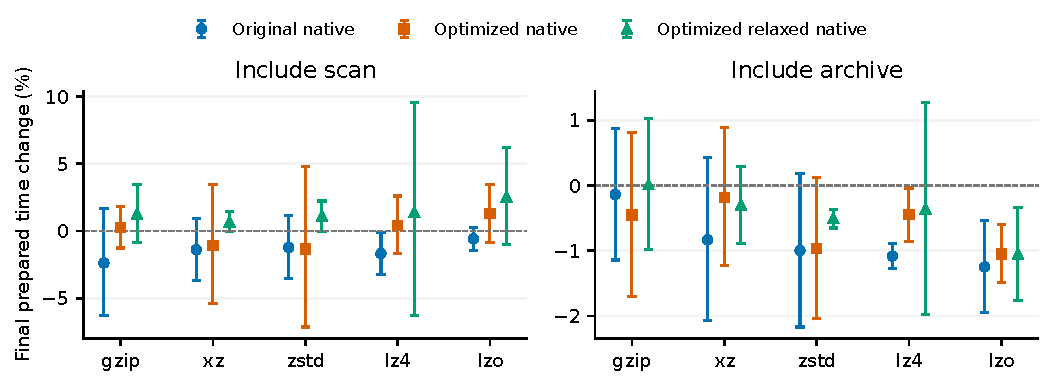
\includegraphics[width=\textwidth]{figures/section65/filesystem-native.pdf}
\caption{Final prepared native versus original, equally optimized normal and
equally optimized relaxed native references. Fresh-mount scan/archive;
pointwise 95\% campaign intervals. Negative values mean lower elapsed time.}
\label{fig:filesystem-native}
\end{figure*}

For the nine nonempty ordinary application tasks, VKSO/copied point estimates range from 0.9901 to 1.0056, with pointwise interval endpoints spanning [0.9584, 1.0255] (Figure~\ref{fig:filesystem-sharing}). Equal-length-path xz/lz4 scan/stream controls have point estimates 0.9608--1.0188 and interval endpoints [0.8435, 1.0945]. The single-CPU gzip-stream change is -0.13\% [-1.02\%, +0.77\%]. The observed interval widths bound the precision of the sharing-cost conclusion; they do not establish universal equivalence.
These comparisons hold the owner instructions, bridge, frontend, cache
policy and translator fixed. Ordinary deployment retains its carrier
paths; the separate xz/lz4 scan/stream diagnostic also equalizes loader-path
lengths. The latter provides the tighter backing control for those four cells.

\begin{figure}[t]\centering
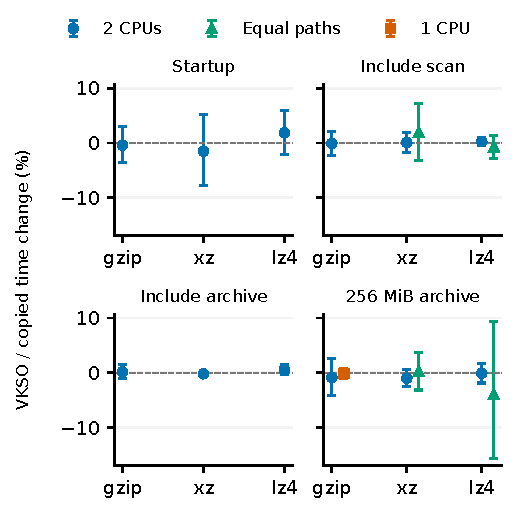
\includegraphics[width=\columnwidth]{figures/section65/filesystem-sharing.pdf}
\caption{VKSO versus identical-core copied execution. All ordinary tasks are
shown; the selected gzip-stream single-CPU check remains a separate condition.
Pointwise 95\% campaign intervals.}
\label{fig:filesystem-sharing}
\end{figure}

\paragraph{Application effects.}
Relative to default SquashFUSE, include-scan elapsed changes range from -54.58\% to -4.42\% and include-archive changes from -19.46\% to -3.30\%. Sequential gzip, xz and lz4 changes are -7.27\% [-10.27\%, -4.17\%], +13.10\% [+11.45\%, +14.78\%], -7.23\% [-11.26\%, -3.02\%], respectively (Figure~\ref{fig:filesystem-application}). Across all twelve ordinary tasks, final VKSO/cache-matched-LKL time ratios range from 0.6323 to 0.9050; the full table retains their per-task intervals.
Against single-thread SquashFUSE, gzip and lz4 include archives instead change by +1.18\% [+0.44\%, +1.93\%] and +0.89\% [+0.65\%, +1.13\%]. The corresponding scans are close in point estimate, whereas xz scan remains faster at -53.59\% [-54.49\%, -52.68\%]. Thus stock threading explains much of the gzip/lz4 metadata advantage over its default configuration, but not the large xz difference.
In a separate xz metadata-work diagnostic, default and single-thread
SquashFUSE each decode 137 blocks and 1,106,363 bytes; the common parser
decodes 76 blocks and 558,231 bytes, whether it uses library or common XZ.
Three replays agree. Reduced decompression work contributes to the metadata
advantage; these counts do not assign the whole time difference to one cause.

\begin{figure*}[t]\centering
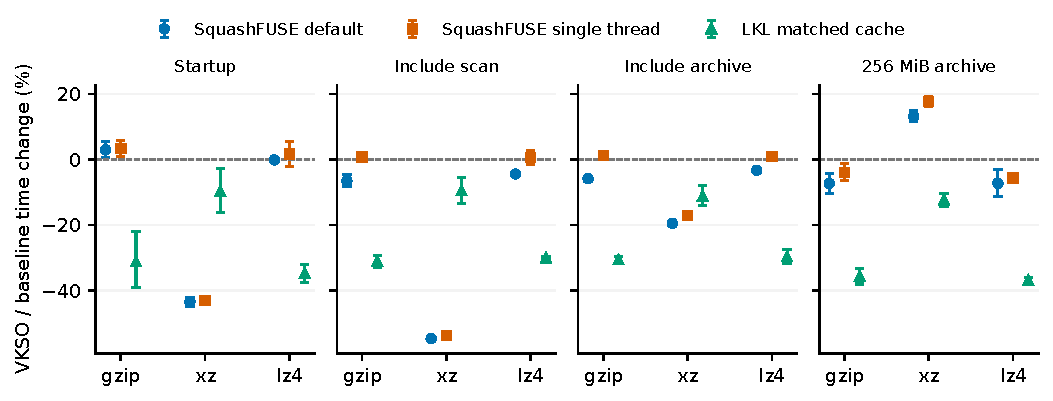
\includegraphics[width=\textwidth]{figures/section65/filesystem-application.pdf}
\caption{Complete VKSO application time relative to default/single-thread
SquashFUSE and cache-matched LKL512. Startup, metadata and sequential tasks
retain their own outcomes and pointwise 95\% intervals.}
\label{fig:filesystem-application}
\end{figure*}

An independent distribution task compiles the Python~3.10 standard library
through real gzip/xz SIFs into a fresh writable bytecode cache. The task and
images were fixed before confirmation and were not used to optimize the
reader. Every backend generates the same 647 bytecode files.
VKSO changes complete compilation time by +0.68\% [+0.22\%, +1.14\%] (gzip) and +16.18\% [+15.56\%, +16.80\%] (xz) relative to default SquashFUSE. Against cache-matched LKL, the changes are -6.05\% [-6.72\%, -5.38\%] and +6.72\% [+6.31\%, +7.13\%], respectively (Figure~\ref{fig:filesystem-heldout}).
This held-out task does not establish a general application speedup: the
additional XZ reuse has a measurable cost, including against LKL for this task.

\begin{figure}[t]\centering
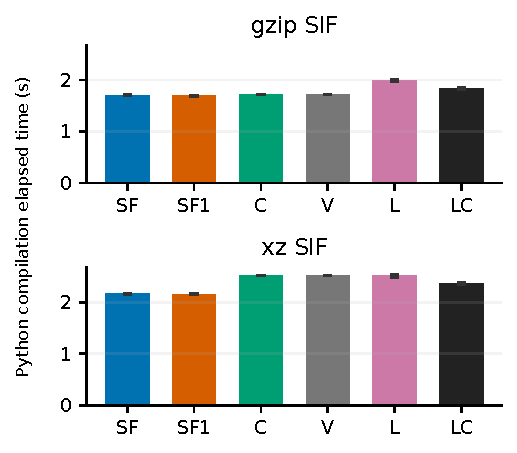
\includegraphics[width=\columnwidth]{figures/section65/filesystem-heldout.pdf}
\caption{Held-out standard-library compilation: mean campaign medians with
pointwise 95\% intervals. SF/SF1: default/single-thread SquashFUSE; C/V:
copied/VKSO; L/LC: default/cache-matched LKL512.}
\label{fig:filesystem-heldout}
\end{figure}

With both external libraries retained, switching from library to common decoding changes xz/lz4 sequential time by +14.79\% [+13.43\%, +16.16\%] / -0.31\% [-2.36\%, +1.78\%]. Removing the now-unused dependencies while retaining common decoding changes it by -0.51\% [-2.45\%, +1.47\%] / +0.89\% [-3.00\%, +4.94\%]. The xz decoder switch changes measured child CPU time by +14.87\%, consistent with an execution-cost difference.
Dependency removal has a small, uncertain effect. The controlled
comparison attributes the final sequential loss primarily to the decoder
execution choice; it does not identify a particular inner-loop cause.
These diagnostics compare library decoding, common decoding with both
libraries retained, and common decoding after dependency removal on the
same owner. They explain final-build tradeoffs without assigning prior
layout-sensitive results to physical sharing.

\paragraph{Engineering and maintenance.}
Reuse preserves the original format/decoder implementations, but requires
explicit preparation and domain support. Sixteen native source/header files
change, largely through extraction and service exposure. Three of the
34 extracted filesystem bodies differ: device-size access, BIO input
handling, and the maintained/bounded-copy helper. Generated kernel support
and contract headers occupy 390 physical lines. The first user integration
contains a 408-line bridge, 154-line POSIX/codec binding and 300-line FUSE
frontend; the application translator adds 96 lines. Generators, reused LZ4
sources, unchanged XZ algorithms and general-exporter fixes are accounted
separately in the artifact. These measures describe maintenance surfaces;
they do not establish reduced developer hours. LKL's SIF integration adds
30 lines to its existing frontend; incremental application adapters are
compared from an existing-platform starting point in both cases.

The known upstream negative-offset repair is reproduced in isolated guests
across old/fixed native, copied and shared paths. The repair changes the
common implementation while preserving the bridge/frontend in that
maintenance experiment. The final composed owner retains the repaired
filesystem source and passes a new guest regression: native/copied/shared
report EIO, user daemons survive, and normal five-format reads, restoration
and unloading pass. A repair requires rebuilding and redeploying the owner;
copied execution receives the same source-maintenance benefit. The shared
XZ hardware breakpoint and the retained ISO9660 replay demonstrate debugging
of common instructions from the user environment.

\paragraph{Resources and deployment.}
After the include archive, VKSO helper PSS is 7.00--7.04~MiB, compared with 14.16--23.95~MiB for default SquashFUSE, 11.64--12.85~MiB for single-thread SquashFUSE, and 82.57--82.85~MiB for cache-matched LKL. In separate untimed metadata-scale runs, VKSO retained PSS is 7.02, 23.43, 88.89~MiB after visiting 5,866, 23,464 and 93,856 entries. At the largest scale, default/single-thread SquashFUSE and cache-matched LKL retain 28.52, 12.91, 500.92~MiB, respectively. The scale result exposes the cost of retaining private metadata; the small-tree footprint is not a fixed runtime-memory bound.
The bridge retains its inode/name lists until unmount and has no eviction
policy. This implementation choice accounts for growth in visited metadata;
the compact-runtime result applies to the small trees, not to all mount sizes.
\begin{table}[t]\centering\small
\caption{Helper PSS after include archive, before PFN observation. Ranges span three codecs and three campaigns; they are not peaks.}
\label{tab:filesystem-resources}
\begin{tabular}{lr}\toprule Backend & PSS range (MiB) \\\midrule
SF & 14.16--23.95 \\
SF1 & 11.64--12.85 \\
C & 6.99--7.04 \\
V & 7.00--7.04 \\
L & 82.53--82.81 \\
LC & 82.57--82.85 \\
\bottomrule\end{tabular}\end{table}

The installed-platform premise treats the generic 32~KiB
\texttt{page\_cache\_replace} module as one-time infrastructure. Filesystem
preparation and per-core registration remain business costs
(Table~\ref{tab:filesystem-business}).
An already prepared native service can avoid one 36~KiB user backing while
requesting 1,264 bytes of registration metadata. Relative to a matched native
module reference, the prepared owner/consumer adds 48~KiB of component residency. User-only
deployment retains the 68~KiB owner; an actual SIF run succeeds without the
native consumer or construction observer, whereas copied execution also
succeeds after all task modules unload. Ordinary copied DSOs share between
user processes, so avoided backing has no process-count multiplier.
\begin{table}[t]\centering\small
\caption{Filesystem component costs with the generic platform installed. Residency, avoided backing and requested metadata are separate quantities.}
\label{tab:filesystem-business}
\begin{tabular}{lr}\toprule Component & Size \\\midrule
Matched native module & 60 KiB \\
Prepared owner + consumer & 108 KiB \\
Native preparation increment & 48 KiB \\
Avoided core backing & 36 KiB \\
Requested registration metadata & 1,264 B \\
\bottomrule\end{tabular}\end{table}

Across nine ordinary application campaigns, core construction, export and registration take a median 2.698~s (observed range [2.696, 6.088]~s), excluding compilation, module loading and validation. This setup is reused by later invocations while the owner and registration remain installed; an owner reload or version change requires fresh deployment. Copied artifact construction also has a setup cost, so these measurements do not assume that its preparation is free.
Module residency, requested allocations and process PSS remain separate
ledgers; the case does not establish whole-machine net-memory savings.

The results support a common resident filesystem/decoder body serving
native and real application consumers with private state and one source
repair point. Complete-backend efficiency and maintenance benefits also
apply to copied execution; VKSO adds native/user physical identity with the
measured incremental cost. Performance conclusions cover these read-only
SIFs and tasks on this host/boot. Five-format functionality, boundary-read
correctness and simultaneous lifetimes do not by themselves establish
five-format application speed, random-I/O performance or concurrent scaling.

\bibliographystyle{plain}
\bibliography{paper_content/references}
\clearpage\onecolumn
\section*{Filesystem evaluation: final-owner results}
\small
The final XZ-composed owner is evaluated in 30 campaigns with
6,540 observations. The table retains all paired comparisons.
Absolute times are means of campaign medians. Ratios instead average paired
log ratios within each campaign and weight the three campaigns equally;
adjacent absolute times therefore need not divide to the paired ratio.
Intervals are pointwise 95\% Student-t intervals over campaign estimates.

O denotes original native, N the equally optimized normal native reference,
NR its relaxed-options counterpart, PL the preceding LZ4-composed owner, and
PX the final XZ-composed owner. SF and SF1 are the same squashfuse\_ll binary
with default and single-thread operation; SF+T adds the common translator.
C and V use identical common instructions with copied and kernel-shared
backing. L and LC are LKL512 with default and matched positive caches.
CL uses library decoders with both libraries present; CR uses common
decoders while retaining both libraries. Their separate diagnostic uses
equal-length loader paths. The single-CPU group is separate from the default
two-CPU application matrix.

\begin{figure}[h]\centering
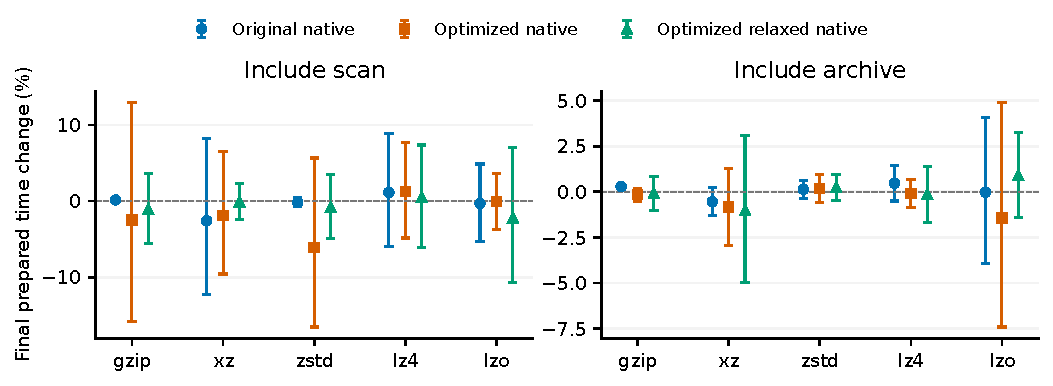
\includegraphics[width=\textwidth]{figures/section65/filesystem-native-warm.pdf}
\caption{Warm traversals after the fresh-mount native task. These accesses
can bypass common-core work and are not the sole preparation-cost evidence.}
\end{figure}
\begin{figure}[h]\centering
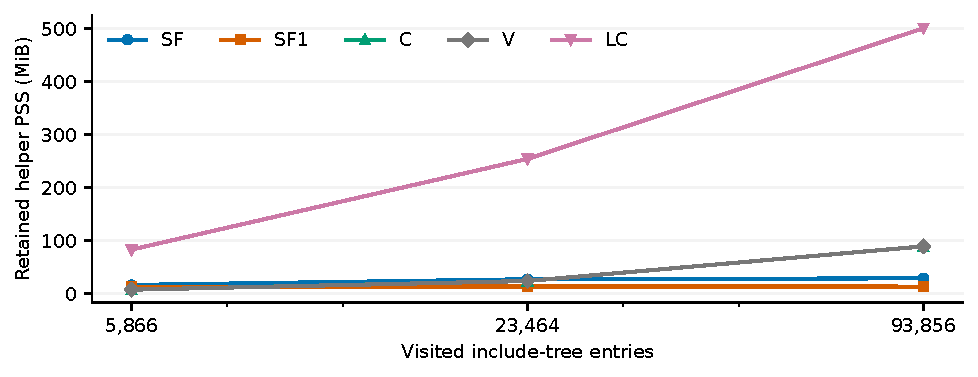
\includegraphics[width=.9\textwidth]{figures/section65/filesystem-memory-scale.pdf}
\caption{Untimed metadata-scale observations after complete include archives.
The tree distribution is replicated with distinct inodes; SquashFS may
deduplicate file data. Each point is one separate process/mount observation,
not a population confidence interval or a whole-machine memory measurement.}
\end{figure}
\clearpage
\section*{Bounded diagnostic evidence}
\begin{table}[h]\centering\small
\caption{Actual object-code audit. The PIC probe is a build-only feasibility check with an explicit GS canary convention; it is not a runnable hardened VKSO configuration.}
\begin{tabular}{lrrr}\toprule Object configuration & GS canary & Indirect thunks & Return thunks \\\midrule
Optimized normal native & yes & yes & yes \\
Optimized relaxed native & no & no & no \\
Final prepared filesystem & no & no & no \\
PIC hardened build-only probe & yes & yes & yes \\
\bottomrule\end{tabular}\end{table}

\begin{table}[h]\centering\small
\caption{Separate mount-and-scan diagnostic. Decoder API work includes mount startup; all three replays agree. Instrumented time is not used.}
\begin{tabular}{lrrr}\toprule Backend & Decoder calls & Input bytes & Decoded bytes \\\midrule
SF & 137 & 376,636 & 1,106,363 \\
SF1 & 137 & 376,636 & 1,106,363 \\
C & 76 & 189,736 & 558,231 \\
CL & 76 & 189,736 & 558,231 \\
\bottomrule\end{tabular}\end{table}

\begin{table}[h]\centering\small
\caption{Exploratory LKL heap pilot: all settings complete all four tasks. Gzip has four blocks; xz/lz4 have one. Times are descriptive medians. PSS follows the include archive, not a sequential-task peak.}
\begin{tabular}{lrrrrrr}\toprule Codec & Heap MiB & Startup s & Scan s & Archive s & Stream s & PSS MiB \\ \midrule
gzip & 16 & 0.239 & 2.041 & 3.384 & 0.941 & 23.08 \\
gzip & 64 & 0.218 & 2.032 & 2.510 & 0.918 & 60.03 \\
gzip & 256 & 0.211 & 2.008 & 2.274 & 0.943 & 78.65 \\
gzip & 512 & 0.233 & 2.052 & 2.194 & 0.932 & 82.54 \\
xz & 16 & 0.269 & 1.031 & 3.985 & 1.251 & 23.12 \\
xz & 64 & 0.288 & 1.065 & 3.059 & 1.178 & 60.15 \\
xz & 256 & 0.284 & 1.044 & 2.866 & 1.236 & 78.84 \\
xz & 512 & 0.302 & 1.055 & 2.772 & 1.223 & 82.72 \\
lz4 & 16 & 0.211 & 1.983 & 3.073 & 0.821 & 23.11 \\
lz4 & 64 & 0.211 & 1.946 & 2.081 & 0.778 & 59.54 \\
lz4 & 256 & 0.238 & 1.972 & 1.999 & 0.774 & 78.90 \\
lz4 & 512 & 0.192 & 1.988 & 1.994 & 0.811 & 82.79 \\
\bottomrule\end{tabular}\end{table}

\clearpage
\setlength{\LTcapwidth}{\linewidth}
\begin{longtable}{lllrrrr}
\toprule
Codec/task/phase & Base & Test & Base s & Test s & Ratio & 95\% CI \\
\midrule\endhead
\multicolumn{7}{l}{\textbf{application final}} \\
gzip/archive/app & C & V & 0.9078 & 0.9065 & 1.0016 & [0.9890, 1.0144] \\
gzip/archive/app & L & LC & 2.2307 & 1.3040 & 0.5790 & [0.5733, 0.5848] \\
gzip/archive/app & L & V & 2.2307 & 0.9065 & 0.4022 & [0.3965, 0.4081] \\
gzip/archive/app & LC & V & 1.3040 & 0.9065 & 0.6946 & [0.6861, 0.7033] \\
gzip/archive/app & SF & C & 0.9626 & 0.9078 & 0.9403 & [0.9279, 0.9528] \\
gzip/archive/app & SF & L & 0.9626 & 2.2307 & 2.3415 & [2.3117, 2.3717] \\
gzip/archive/app & SF & LC & 0.9626 & 1.3040 & 1.3558 & [1.3336, 1.3783] \\
gzip/archive/app & SF & SF1 & 0.9626 & 0.8992 & 0.9308 & [0.9249, 0.9367] \\
gzip/archive/app & SF & SF+T & 0.9626 & 0.9613 & 0.9981 & [0.9864, 1.0099] \\
gzip/archive/app & SF & V & 0.9626 & 0.9065 & 0.9418 & [0.9341, 0.9495] \\
gzip/archive/app & SF1 & V & 0.8992 & 0.9065 & 1.0118 & [1.0044, 1.0193] \\
gzip/scan/app & C & V & 0.4568 & 0.4578 & 0.9992 & [0.9774, 1.0215] \\
gzip/scan/app & L & LC & 2.0241 & 0.6641 & 0.3283 & [0.3230, 0.3337] \\
gzip/scan/app & L & V & 2.0241 & 0.4578 & 0.2263 & [0.2233, 0.2294] \\
gzip/scan/app & LC & V & 0.6641 & 0.4578 & 0.6893 & [0.6713, 0.7079] \\
gzip/scan/app & SF & C & 0.4887 & 0.4568 & 0.9355 & [0.9128, 0.9587] \\
gzip/scan/app & SF & L & 0.4887 & 2.0241 & 4.1305 & [4.0997, 4.1616] \\
gzip/scan/app & SF & LC & 0.4887 & 0.6641 & 1.3560 & [1.3440, 1.3681] \\
gzip/scan/app & SF & SF1 & 0.4887 & 0.4536 & 0.9273 & [0.9125, 0.9423] \\
gzip/scan/app & SF & SF+T & 0.4887 & 0.4875 & 1.0043 & [1.0020, 1.0067] \\
gzip/scan/app & SF & V & 0.4887 & 0.4578 & 0.9347 & [0.9168, 0.9530] \\
gzip/scan/app & SF1 & V & 0.4536 & 0.4578 & 1.0080 & [0.9998, 1.0163] \\
gzip/startup/app & C & V & 0.1480 & 0.1472 & 0.9958 & [0.9634, 1.0293] \\
gzip/startup/app & L & LC & 0.2304 & 0.2152 & 0.9574 & [0.8647, 1.0600] \\
gzip/startup/app & L & V & 0.2304 & 0.1472 & 0.6597 & [0.6059, 0.7182] \\
gzip/startup/app & LC & V & 0.2152 & 0.1472 & 0.6890 & [0.6091, 0.7794] \\
gzip/startup/app & SF & C & 0.1442 & 0.1480 & 1.0339 & [1.0226, 1.0454] \\
gzip/startup/app & SF & L & 0.1442 & 0.2304 & 1.5608 & [1.4550, 1.6742] \\
gzip/startup/app & SF & LC & 0.1442 & 0.2152 & 1.4943 & [1.3514, 1.6523] \\
gzip/startup/app & SF & SF1 & 0.1442 & 0.1430 & 0.9966 & [0.9810, 1.0125] \\
gzip/startup/app & SF & SF+T & 0.1442 & 0.1449 & 1.0088 & [0.9608, 1.0592] \\
gzip/startup/app & SF & V & 0.1442 & 0.1472 & 1.0296 & [1.0059, 1.0538] \\
gzip/startup/app & SF1 & V & 0.1430 & 0.1472 & 1.0331 & [1.0097, 1.0570] \\
gzip/stream/app & C & V & 0.6124 & 0.6104 & 0.9914 & [0.9584, 1.0255] \\
gzip/stream/app & L & LC & 0.9582 & 0.9466 & 0.9894 & [0.9734, 1.0057] \\
gzip/stream/app & L & V & 0.9582 & 0.6104 & 0.6370 & [0.6231, 0.6513] \\
gzip/stream/app & LC & V & 0.9466 & 0.6104 & 0.6438 & [0.6208, 0.6677] \\
gzip/stream/app & SF & C & 0.6533 & 0.6124 & 0.9353 & [0.9336, 0.9370] \\
gzip/stream/app & SF & L & 0.6533 & 0.9582 & 1.4556 & [1.4378, 1.4737] \\
gzip/stream/app & SF & LC & 0.6533 & 0.9466 & 1.4402 & [1.4345, 1.4460] \\
gzip/stream/app & SF & SF1 & 0.6533 & 0.6297 & 0.9650 & [0.9521, 0.9782] \\
gzip/stream/app & SF & SF+T & 0.6533 & 0.6527 & 0.9934 & [0.9829, 1.0041] \\
gzip/stream/app & SF & V & 0.6533 & 0.6104 & 0.9273 & [0.8973, 0.9583] \\
gzip/stream/app & SF1 & V & 0.6297 & 0.6104 & 0.9609 & [0.9356, 0.9868] \\
lz4/archive/app & C & V & 0.7873 & 0.7864 & 1.0056 & [0.9965, 1.0149] \\
lz4/archive/app & L & LC & 2.0402 & 1.1235 & 0.5460 & [0.5330, 0.5592] \\
lz4/archive/app & L & V & 2.0402 & 0.7864 & 0.3843 & [0.3790, 0.3895] \\
lz4/archive/app & LC & V & 1.1235 & 0.7864 & 0.7038 & [0.6828, 0.7255] \\
lz4/archive/app & SF & C & 0.8158 & 0.7873 & 0.9616 & [0.9491, 0.9743] \\
lz4/archive/app & SF & L & 0.8158 & 2.0402 & 2.5166 & [2.4971, 2.5363] \\
lz4/archive/app & SF & LC & 0.8158 & 1.1235 & 1.3740 & [1.3347, 1.4144] \\
lz4/archive/app & SF & SF1 & 0.8158 & 0.7818 & 0.9585 & [0.9521, 0.9649] \\
lz4/archive/app & SF & SF+T & 0.8158 & 0.8145 & 0.9976 & [0.9880, 1.0072] \\
lz4/archive/app & SF & V & 0.8158 & 0.7864 & 0.9670 & [0.9604, 0.9737] \\
lz4/archive/app & SF1 & V & 0.7818 & 0.7864 & 1.0089 & [1.0065, 1.0113] \\
lz4/scan/app & C & V & 0.4384 & 0.4386 & 1.0021 & [0.9946, 1.0096] \\
lz4/scan/app & L & LC & 1.9684 & 0.6306 & 0.3199 & [0.3114, 0.3285] \\
lz4/scan/app & L & V & 1.9684 & 0.4386 & 0.2237 & [0.2192, 0.2284] \\
lz4/scan/app & LC & V & 0.6306 & 0.4386 & 0.6995 & [0.6948, 0.7042] \\
lz4/scan/app & SF & C & 0.4612 & 0.4384 & 0.9538 & [0.9413, 0.9666] \\
lz4/scan/app & SF & L & 0.4612 & 1.9684 & 4.2721 & [4.2030, 4.3423] \\
lz4/scan/app & SF & LC & 0.4612 & 0.6306 & 1.3664 & [1.3485, 1.3846] \\
lz4/scan/app & SF & SF1 & 0.4612 & 0.4374 & 0.9505 & [0.9359, 0.9654] \\
lz4/scan/app & SF & SF+T & 0.4612 & 0.4616 & 1.0008 & [0.9909, 1.0107] \\
lz4/scan/app & SF & V & 0.4612 & 0.4386 & 0.9558 & [0.9495, 0.9621] \\
lz4/scan/app & SF1 & V & 0.4374 & 0.4386 & 1.0056 & [0.9846, 1.0270] \\
lz4/startup/app & C & V & 0.1285 & 0.1296 & 1.0185 & [0.9796, 1.0589] \\
lz4/startup/app & L & LC & 0.2186 & 0.2016 & 0.9339 & [0.9194, 0.9486] \\
lz4/startup/app & L & V & 0.2186 & 0.1296 & 0.6093 & [0.5750, 0.6457] \\
lz4/startup/app & LC & V & 0.2016 & 0.1296 & 0.6524 & [0.6252, 0.6809] \\
lz4/startup/app & SF & C & 0.1297 & 0.1285 & 0.9805 & [0.9357, 1.0275] \\
lz4/startup/app & SF & L & 0.1297 & 0.2186 & 1.6391 & [1.5340, 1.7514] \\
lz4/startup/app & SF & LC & 0.1297 & 0.2016 & 1.5307 & [1.4545, 1.6108] \\
lz4/startup/app & SF & SF1 & 0.1297 & 0.1290 & 0.9821 & [0.9399, 1.0262] \\
lz4/startup/app & SF & SF+T & 0.1297 & 0.1307 & 1.0086 & [0.9496, 1.0713] \\
lz4/startup/app & SF & V & 0.1297 & 0.1296 & 0.9987 & [0.9902, 1.0072] \\
lz4/startup/app & SF1 & V & 0.1290 & 0.1296 & 1.0168 & [0.9792, 1.0559] \\
lz4/stream/app & C & V & 0.5022 & 0.5020 & 0.9990 & [0.9813, 1.0171] \\
lz4/stream/app & L & LC & 0.7996 & 0.7919 & 0.9935 & [0.9805, 1.0066] \\
lz4/stream/app & L & V & 0.7996 & 0.5020 & 0.6282 & [0.6138, 0.6429] \\
lz4/stream/app & LC & V & 0.7919 & 0.5020 & 0.6323 & [0.6235, 0.6413] \\
lz4/stream/app & SF & C & 0.5454 & 0.5022 & 0.9285 & [0.8724, 0.9883] \\
lz4/stream/app & SF & L & 0.5454 & 0.7996 & 1.4767 & [1.4233, 1.5322] \\
lz4/stream/app & SF & LC & 0.5454 & 0.7919 & 1.4671 & [1.4016, 1.5357] \\
lz4/stream/app & SF & SF1 & 0.5454 & 0.5315 & 0.9825 & [0.9375, 1.0296] \\
lz4/stream/app & SF & SF+T & 0.5454 & 0.5455 & 1.0120 & [0.9592, 1.0677] \\
lz4/stream/app & SF & V & 0.5454 & 0.5020 & 0.9277 & [0.8874, 0.9698] \\
lz4/stream/app & SF1 & V & 0.5315 & 0.5020 & 0.9442 & [0.9368, 0.9516] \\
xz/archive/app & C & V & 1.6456 & 1.6436 & 0.9981 & [0.9937, 1.0025] \\
xz/archive/app & L & LC & 2.5984 & 1.8451 & 0.7024 & [0.6861, 0.7190] \\
xz/archive/app & L & V & 2.5984 & 1.6436 & 0.6243 & [0.5898, 0.6607] \\
xz/archive/app & LC & V & 1.8451 & 1.6436 & 0.8888 & [0.8592, 0.9194] \\
xz/archive/app & SF & C & 2.0403 & 1.6456 & 0.8069 & [0.8048, 0.8090] \\
xz/archive/app & SF & L & 2.0403 & 2.5984 & 1.2901 & [1.2227, 1.3611] \\
xz/archive/app & SF & LC & 2.0403 & 1.8451 & 0.9061 & [0.8789, 0.9342] \\
xz/archive/app & SF & SF1 & 2.0403 & 1.9817 & 0.9712 & [0.9660, 0.9765] \\
xz/archive/app & SF & SF+T & 2.0403 & 2.0419 & 0.9998 & [0.9983, 1.0013] \\
xz/archive/app & SF & V & 2.0403 & 1.6436 & 0.8054 & [0.8022, 0.8085] \\
xz/archive/app & SF1 & V & 1.9817 & 1.6436 & 0.8292 & [0.8216, 0.8370] \\
xz/scan/app & C & V & 0.5850 & 0.5851 & 1.0007 & [0.9828, 1.0189] \\
xz/scan/app & L & LC & 1.0711 & 0.6443 & 0.6070 & [0.5950, 0.6192] \\
xz/scan/app & L & V & 1.0711 & 0.5851 & 0.5493 & [0.5327, 0.5665] \\
xz/scan/app & LC & V & 0.6443 & 0.5851 & 0.9050 & [0.8657, 0.9461] \\
xz/scan/app & SF & C & 1.2954 & 0.5850 & 0.4539 & [0.4523, 0.4555] \\
xz/scan/app & SF & L & 1.2954 & 1.0711 & 0.8269 & [0.8149, 0.8390] \\
xz/scan/app & SF & LC & 1.2954 & 0.6443 & 0.5019 & [0.4875, 0.5168] \\
xz/scan/app & SF & SF1 & 1.2954 & 1.2692 & 0.9788 & [0.9723, 0.9854] \\
xz/scan/app & SF & SF+T & 1.2954 & 1.2943 & 1.0003 & [0.9915, 1.0092] \\
xz/scan/app & SF & V & 1.2954 & 0.5851 & 0.4542 & [0.4469, 0.4617] \\
xz/scan/app & SF1 & V & 1.2692 & 0.5851 & 0.4641 & [0.4551, 0.4732] \\
xz/startup/app & C & V & 0.2558 & 0.2565 & 0.9847 & [0.9222, 1.0514] \\
xz/startup/app & L & LC & 0.2993 & 0.2814 & 0.9493 & [0.8461, 1.0650] \\
xz/startup/app & L & V & 0.2993 & 0.2565 & 0.8572 & [0.8222, 0.8937] \\
xz/startup/app & LC & V & 0.2814 & 0.2565 & 0.9030 & [0.8385, 0.9724] \\
xz/startup/app & SF & C & 0.4547 & 0.2558 & 0.5754 & [0.5454, 0.6069] \\
xz/startup/app & SF & L & 0.4547 & 0.2993 & 0.6610 & [0.6468, 0.6754] \\
xz/startup/app & SF & LC & 0.4547 & 0.2814 & 0.6274 & [0.5709, 0.6895] \\
xz/startup/app & SF & SF1 & 0.4547 & 0.4504 & 0.9933 & [0.9634, 1.0242] \\
xz/startup/app & SF & SF+T & 0.4547 & 0.4551 & 1.0050 & [0.9718, 1.0394] \\
xz/startup/app & SF & V & 0.4547 & 0.2565 & 0.5666 & [0.5534, 0.5801] \\
xz/startup/app & SF1 & V & 0.4504 & 0.2565 & 0.5704 & [0.5652, 0.5756] \\
xz/stream/app & C & V & 1.0799 & 1.0778 & 0.9901 & [0.9747, 1.0057] \\
xz/stream/app & L & LC & 1.2355 & 1.2221 & 0.9919 & [0.9886, 0.9951] \\
xz/stream/app & L & V & 1.2355 & 1.0778 & 0.8695 & [0.8523, 0.8870] \\
xz/stream/app & LC & V & 1.2221 & 1.0778 & 0.8766 & [0.8566, 0.8971] \\
xz/stream/app & SF & C & 0.9469 & 1.0799 & 1.1423 & [1.1308, 1.1541] \\
xz/stream/app & SF & L & 0.9469 & 1.2355 & 1.3008 & [1.2924, 1.3093] \\
xz/stream/app & SF & LC & 0.9469 & 1.2221 & 1.2902 & [1.2786, 1.3020] \\
xz/stream/app & SF & SF1 & 0.9469 & 0.9120 & 0.9616 & [0.9558, 0.9674] \\
xz/stream/app & SF & SF+T & 0.9469 & 0.9450 & 0.9959 & [0.9885, 1.0033] \\
xz/stream/app & SF & V & 0.9469 & 1.0778 & 1.1310 & [1.1145, 1.1478] \\
xz/stream/app & SF1 & V & 0.9120 & 1.0778 & 1.1762 & [1.1623, 1.1903] \\
\multicolumn{7}{l}{\textbf{decoder diagnostic}} \\
lz4/scan/app & C & V & 0.4416 & 0.4381 & 0.9926 & [0.9714, 1.0143] \\
lz4/scan/app & CL & C & 0.4411 & 0.4416 & 1.0079 & [0.9870, 1.0293] \\
lz4/scan/app & CL & CR & 0.4411 & 0.4408 & 0.9984 & [0.9928, 1.0040] \\
lz4/scan/app & CR & C & 0.4408 & 0.4416 & 1.0095 & [0.9917, 1.0277] \\
lz4/scan/app & SF & C & 0.4627 & 0.4416 & 0.9598 & [0.9371, 0.9831] \\
lz4/scan/app & SF & CL & 0.4627 & 0.4411 & 0.9523 & [0.9395, 0.9652] \\
lz4/scan/app & SF & CR & 0.4627 & 0.4408 & 0.9508 & [0.9418, 0.9599] \\
lz4/scan/app & SF & V & 0.4627 & 0.4381 & 0.9528 & [0.9304, 0.9757] \\
lz4/stream/app & C & V & 0.4971 & 0.4939 & 0.9608 & [0.8435, 1.0945] \\
lz4/stream/app & CL & C & 0.4944 & 0.4971 & 1.0058 & [0.9837, 1.0283] \\
lz4/stream/app & CL & CR & 0.4944 & 0.4937 & 0.9969 & [0.9764, 1.0178] \\
lz4/stream/app & CR & C & 0.4937 & 0.4971 & 1.0089 & [0.9700, 1.0494] \\
lz4/stream/app & SF & C & 0.5379 & 0.4971 & 0.9501 & [0.8212, 1.0993] \\
lz4/stream/app & SF & CL & 0.5379 & 0.4944 & 0.9447 & [0.8347, 1.0692] \\
lz4/stream/app & SF & CR & 0.5379 & 0.4937 & 0.9417 & [0.8449, 1.0496] \\
lz4/stream/app & SF & V & 0.5379 & 0.4939 & 0.9129 & [0.7307, 1.1406] \\
xz/scan/app & C & V & 0.5844 & 0.6007 & 1.0188 & [0.9687, 1.0716] \\
xz/scan/app & CL & C & 0.5768 & 0.5844 & 1.0043 & [0.9779, 1.0315] \\
xz/scan/app & CL & CR & 0.5768 & 0.5856 & 1.0050 & [0.9737, 1.0372] \\
xz/scan/app & CR & C & 0.5856 & 0.5844 & 0.9994 & [0.9944, 1.0043] \\
xz/scan/app & SF & C & 1.3112 & 0.5844 & 0.4495 & [0.4428, 0.4564] \\
xz/scan/app & SF & CL & 1.3112 & 0.5768 & 0.4476 & [0.4400, 0.4554] \\
xz/scan/app & SF & CR & 1.3112 & 0.5856 & 0.4498 & [0.4413, 0.4586] \\
xz/scan/app & SF & V & 1.3112 & 0.6007 & 0.4580 & [0.4421, 0.4745] \\
xz/stream/app & C & V & 1.0657 & 1.0696 & 1.0026 & [0.9685, 1.0378] \\
xz/stream/app & CL & C & 0.9364 & 1.0657 & 1.1420 & [1.1301, 1.1541] \\
xz/stream/app & CL & CR & 0.9364 & 1.0681 & 1.1479 & [1.1343, 1.1616] \\
xz/stream/app & CR & C & 1.0681 & 1.0657 & 0.9949 & [0.9755, 1.0147] \\
xz/stream/app & SF & C & 0.9463 & 1.0657 & 1.1197 & [1.0325, 1.2143] \\
xz/stream/app & SF & CL & 0.9463 & 0.9364 & 0.9805 & [0.9024, 1.0653] \\
xz/stream/app & SF & CR & 0.9463 & 1.0681 & 1.1255 & [1.0438, 1.2136] \\
xz/stream/app & SF & V & 0.9463 & 1.0696 & 1.1226 & [1.0715, 1.1761] \\
\multicolumn{7}{l}{\textbf{heldout}} \\
gzip/compile/app & C & V & 1.7185 & 1.7162 & 0.9943 & [0.9891, 0.9995] \\
gzip/compile/app & L & LC & 1.9863 & 1.8270 & 0.9159 & [0.9110, 0.9208] \\
gzip/compile/app & L & V & 1.9863 & 1.7162 & 0.8605 & [0.8572, 0.8637] \\
gzip/compile/app & LC & V & 1.8270 & 1.7162 & 0.9395 & [0.9328, 0.9462] \\
gzip/compile/app & SF & C & 1.7014 & 1.7185 & 1.0126 & [1.0108, 1.0144] \\
gzip/compile/app & SF & L & 1.7014 & 1.9863 & 1.1700 & [1.1611, 1.1790] \\
gzip/compile/app & SF & LC & 1.7014 & 1.8270 & 1.0717 & [1.0592, 1.0843] \\
gzip/compile/app & SF & SF1 & 1.7014 & 1.6920 & 0.9924 & [0.9809, 1.0041] \\
gzip/compile/app & SF & V & 1.7014 & 1.7162 & 1.0068 & [1.0022, 1.0114] \\
gzip/compile/app & SF1 & V & 1.6920 & 1.7162 & 1.0144 & [1.0072, 1.0217] \\
xz/compile/app & C & V & 2.5199 & 2.5179 & 0.9991 & [0.9934, 1.0049] \\
xz/compile/app & L & LC & 2.5138 & 2.3632 & 0.9385 & [0.9285, 0.9486] \\
xz/compile/app & L & V & 2.5138 & 2.5179 & 1.0016 & [0.9886, 1.0148] \\
xz/compile/app & LC & V & 2.3632 & 2.5179 & 1.0672 & [1.0631, 1.0713] \\
xz/compile/app & SF & C & 2.1689 & 2.5199 & 1.1628 & [1.1566, 1.1690] \\
xz/compile/app & SF & L & 2.1689 & 2.5138 & 1.1599 & [1.1486, 1.1714] \\
xz/compile/app & SF & LC & 2.1689 & 2.3632 & 1.0886 & [1.0870, 1.0903] \\
xz/compile/app & SF & SF1 & 2.1689 & 2.1577 & 0.9950 & [0.9927, 0.9974] \\
xz/compile/app & SF & V & 2.1689 & 2.5179 & 1.1618 & [1.1556, 1.1680] \\
xz/compile/app & SF1 & V & 2.1577 & 2.5179 & 1.1676 & [1.1592, 1.1760] \\
\multicolumn{7}{l}{\textbf{native final}} \\
gzip/archive/fresh & N & PL & 0.2762 & 0.2745 & 0.9934 & [0.9874, 0.9994] \\
gzip/archive/fresh & N & PX & 0.2762 & 0.2744 & 0.9955 & [0.9829, 1.0082] \\
gzip/archive/fresh & NR & PL & 0.2752 & 0.2745 & 0.9981 & [0.9942, 1.0020] \\
gzip/archive/fresh & NR & PX & 0.2752 & 0.2744 & 1.0002 & [0.9902, 1.0102] \\
gzip/archive/fresh & O & N & 0.2753 & 0.2762 & 1.0032 & [1.0000, 1.0064] \\
gzip/archive/fresh & O & NR & 0.2753 & 0.2752 & 0.9985 & [0.9973, 0.9996] \\
gzip/archive/fresh & O & PL & 0.2753 & 0.2745 & 0.9966 & [0.9937, 0.9995] \\
gzip/archive/fresh & O & PX & 0.2753 & 0.2744 & 0.9986 & [0.9886, 1.0088] \\
gzip/archive/fresh & PL & PX & 0.2745 & 0.2744 & 1.0020 & [0.9930, 1.0112] \\
gzip/archive/warm & N & PL & 0.0538 & 0.0539 & 0.9985 & [0.9912, 1.0060] \\
gzip/archive/warm & N & PX & 0.0538 & 0.0538 & 0.9984 & [0.9949, 1.0018] \\
gzip/archive/warm & NR & PL & 0.0538 & 0.0539 & 0.9993 & [0.9936, 1.0051] \\
gzip/archive/warm & NR & PX & 0.0538 & 0.0538 & 0.9991 & [0.9899, 1.0085] \\
gzip/archive/warm & O & N & 0.0538 & 0.0538 & 1.0045 & [1.0005, 1.0086] \\
gzip/archive/warm & O & NR & 0.0538 & 0.0538 & 1.0037 & [0.9939, 1.0136] \\
gzip/archive/warm & O & PL & 0.0538 & 0.0539 & 1.0031 & [0.9940, 1.0122] \\
gzip/archive/warm & O & PX & 0.0538 & 0.0538 & 1.0029 & [1.0023, 1.0035] \\
gzip/archive/warm & PL & PX & 0.0539 & 0.0538 & 0.9998 & [0.9911, 1.0086] \\
gzip/scan/fresh & N & PL & 0.0628 & 0.0633 & 1.0098 & [0.9883, 1.0318] \\
gzip/scan/fresh & N & PX & 0.0628 & 0.0630 & 1.0027 & [0.9873, 1.0182] \\
gzip/scan/fresh & NR & PL & 0.0618 & 0.0633 & 1.0198 & [1.0064, 1.0333] \\
gzip/scan/fresh & NR & PX & 0.0618 & 0.0630 & 1.0126 & [0.9913, 1.0343] \\
gzip/scan/fresh & O & N & 0.0638 & 0.0628 & 0.9737 & [0.9325, 1.0167] \\
gzip/scan/fresh & O & NR & 0.0638 & 0.0618 & 0.9642 & [0.9321, 0.9974] \\
gzip/scan/fresh & O & PL & 0.0638 & 0.0633 & 0.9832 & [0.9622, 1.0048] \\
gzip/scan/fresh & O & PX & 0.0638 & 0.0630 & 0.9763 & [0.9374, 1.0167] \\
gzip/scan/fresh & PL & PX & 0.0633 & 0.0630 & 0.9929 & [0.9716, 1.0147] \\
gzip/scan/warm & N & PL & 0.0140 & 0.0140 & 0.9883 & [0.8475, 1.1525] \\
gzip/scan/warm & N & PX & 0.0140 & 0.0140 & 0.9750 & [0.8413, 1.1299] \\
gzip/scan/warm & NR & PL & 0.0139 & 0.0140 & 1.0027 & [0.9465, 1.0623] \\
gzip/scan/warm & NR & PX & 0.0139 & 0.0140 & 0.9892 & [0.9444, 1.0360] \\
gzip/scan/warm & O & N & 0.0140 & 0.0140 & 1.0271 & [0.8849, 1.1921] \\
gzip/scan/warm & O & NR & 0.0140 & 0.0139 & 1.0124 & [0.9651, 1.0619] \\
gzip/scan/warm & O & PL & 0.0140 & 0.0140 & 1.0151 & [1.0013, 1.0291] \\
gzip/scan/warm & O & PX & 0.0140 & 0.0140 & 1.0014 & [0.9999, 1.0029] \\
gzip/scan/warm & PL & PX & 0.0140 & 0.0140 & 0.9865 & [0.9723, 1.0009] \\
lz4/archive/fresh & N & PL & 0.1377 & 0.1370 & 0.9955 & [0.9895, 1.0015] \\
lz4/archive/fresh & N & PX & 0.1377 & 0.1369 & 0.9955 & [0.9914, 0.9996] \\
lz4/archive/fresh & NR & PL & 0.1372 & 0.1370 & 0.9964 & [0.9806, 1.0124] \\
lz4/archive/fresh & NR & PX & 0.1372 & 0.1369 & 0.9964 & [0.9802, 1.0128] \\
lz4/archive/fresh & O & N & 0.1387 & 0.1377 & 0.9936 & [0.9904, 0.9969] \\
lz4/archive/fresh & O & NR & 0.1387 & 0.1372 & 0.9928 & [0.9786, 1.0072] \\
lz4/archive/fresh & O & PL & 0.1387 & 0.1370 & 0.9892 & [0.9803, 0.9981] \\
lz4/archive/fresh & O & PX & 0.1387 & 0.1369 & 0.9892 & [0.9872, 0.9911] \\
lz4/archive/fresh & PL & PX & 0.1370 & 0.1369 & 1.0000 & [0.9911, 1.0090] \\
lz4/archive/warm & N & PL & 0.0529 & 0.0529 & 0.9951 & [0.9837, 1.0067] \\
lz4/archive/warm & N & PX & 0.0529 & 0.0529 & 0.9990 & [0.9912, 1.0069] \\
lz4/archive/warm & NR & PL & 0.0530 & 0.0529 & 0.9945 & [0.9827, 1.0065] \\
lz4/archive/warm & NR & PX & 0.0530 & 0.0529 & 0.9984 & [0.9833, 1.0137] \\
lz4/archive/warm & O & N & 0.0527 & 0.0529 & 1.0056 & [0.9938, 1.0176] \\
lz4/archive/warm & O & NR & 0.0527 & 0.0530 & 1.0063 & [1.0000, 1.0126] \\
lz4/archive/warm & O & PL & 0.0527 & 0.0529 & 1.0007 & [0.9929, 1.0086] \\
lz4/archive/warm & O & PX & 0.0527 & 0.0529 & 1.0047 & [0.9950, 1.0144] \\
lz4/archive/warm & PL & PX & 0.0529 & 0.0529 & 1.0039 & [0.9993, 1.0085] \\
lz4/scan/fresh & N & PL & 0.0594 & 0.0597 & 1.0018 & [0.9897, 1.0140] \\
lz4/scan/fresh & N & PX & 0.0594 & 0.0595 & 1.0042 & [0.9830, 1.0260] \\
lz4/scan/fresh & NR & PL & 0.0585 & 0.0597 & 1.0110 & [0.9586, 1.0663] \\
lz4/scan/fresh & NR & PX & 0.0585 & 0.0595 & 1.0135 & [0.9375, 1.0958] \\
lz4/scan/fresh & O & N & 0.0605 & 0.0594 & 0.9790 & [0.9677, 0.9904] \\
lz4/scan/fresh & O & NR & 0.0605 & 0.0585 & 0.9700 & [0.8987, 1.0470] \\
lz4/scan/fresh & O & PL & 0.0605 & 0.0597 & 0.9807 & [0.9577, 1.0042] \\
lz4/scan/fresh & O & PX & 0.0605 & 0.0595 & 0.9831 & [0.9679, 0.9986] \\
lz4/scan/fresh & PL & PX & 0.0597 & 0.0595 & 1.0025 & [0.9722, 1.0337] \\
lz4/scan/warm & N & PL & 0.0129 & 0.0129 & 1.0085 & [0.9700, 1.0486] \\
lz4/scan/warm & N & PX & 0.0129 & 0.0130 & 1.0123 & [0.9514, 1.0771] \\
lz4/scan/warm & NR & PL & 0.0129 & 0.0129 & 1.0006 & [0.9778, 1.0238] \\
lz4/scan/warm & NR & PX & 0.0129 & 0.0130 & 1.0043 & [0.9396, 1.0735] \\
lz4/scan/warm & O & N & 0.0129 & 0.0129 & 0.9991 & [0.9836, 1.0149] \\
lz4/scan/warm & O & NR & 0.0129 & 0.0129 & 1.0071 & [0.9541, 1.0630] \\
lz4/scan/warm & O & PL & 0.0129 & 0.0129 & 1.0076 & [0.9603, 1.0573] \\
lz4/scan/warm & O & PX & 0.0129 & 0.0130 & 1.0114 & [0.9400, 1.0883] \\
lz4/scan/warm & PL & PX & 0.0129 & 0.0130 & 1.0038 & [0.9221, 1.0927] \\
lzo/archive/fresh & N & PL & 0.1539 & 0.1526 & 0.9924 & [0.9804, 1.0045] \\
lzo/archive/fresh & N & PX & 0.1539 & 0.1523 & 0.9895 & [0.9851, 0.9940] \\
lzo/archive/fresh & NR & PL & 0.1531 & 0.1526 & 0.9923 & [0.9830, 1.0016] \\
lzo/archive/fresh & NR & PX & 0.1531 & 0.1523 & 0.9894 & [0.9824, 0.9966] \\
lzo/archive/fresh & O & N & 0.1541 & 0.1539 & 0.9980 & [0.9911, 1.0049] \\
lzo/archive/fresh & O & NR & 0.1541 & 0.1531 & 0.9980 & [0.9952, 1.0009] \\
lzo/archive/fresh & O & PL & 0.1541 & 0.1526 & 0.9903 & [0.9839, 0.9968] \\
lzo/archive/fresh & O & PX & 0.1541 & 0.1523 & 0.9875 & [0.9805, 0.9946] \\
lzo/archive/fresh & PL & PX & 0.1526 & 0.1523 & 0.9971 & [0.9874, 1.0070] \\
lzo/archive/warm & N & PL & 0.0530 & 0.0530 & 0.9815 & [0.8993, 1.0712] \\
lzo/archive/warm & N & PX & 0.0530 & 0.0530 & 0.9856 & [0.9258, 1.0492] \\
lzo/archive/warm & NR & PL & 0.0529 & 0.0530 & 1.0047 & [1.0017, 1.0077] \\
lzo/archive/warm & NR & PX & 0.0529 & 0.0530 & 1.0089 & [0.9859, 1.0323] \\
lzo/archive/warm & O & N & 0.0530 & 0.0530 & 1.0144 & [0.9186, 1.1201] \\
lzo/archive/warm & O & NR & 0.0530 & 0.0529 & 0.9910 & [0.9630, 1.0198] \\
lzo/archive/warm & O & PL & 0.0530 & 0.0530 & 0.9956 & [0.9699, 1.0220] \\
lzo/archive/warm & O & PX & 0.0530 & 0.0530 & 0.9998 & [0.9605, 1.0406] \\
lzo/archive/warm & PL & PX & 0.0530 & 0.0530 & 1.0042 & [0.9793, 1.0297] \\
lzo/scan/fresh & N & PL & 0.0596 & 0.0602 & 1.0099 & [1.0078, 1.0121] \\
lzo/scan/fresh & N & PX & 0.0596 & 0.0602 & 1.0129 & [0.9915, 1.0347] \\
lzo/scan/fresh & NR & PL & 0.0590 & 0.0602 & 1.0223 & [1.0059, 1.0390] \\
lzo/scan/fresh & NR & PX & 0.0590 & 0.0602 & 1.0253 & [0.9898, 1.0620] \\
lzo/scan/fresh & O & N & 0.0608 & 0.0596 & 0.9815 & [0.9683, 0.9949] \\
lzo/scan/fresh & O & NR & 0.0608 & 0.0590 & 0.9697 & [0.9425, 0.9975] \\
lzo/scan/fresh & O & PL & 0.0608 & 0.0602 & 0.9912 & [0.9793, 1.0034] \\
lzo/scan/fresh & O & PX & 0.0608 & 0.0602 & 0.9941 & [0.9856, 1.0027] \\
lzo/scan/fresh & PL & PX & 0.0602 & 0.0602 & 1.0029 & [0.9835, 1.0227] \\
lzo/scan/warm & N & PL & 0.0131 & 0.0131 & 1.0026 & [0.9812, 1.0244] \\
lzo/scan/warm & N & PX & 0.0131 & 0.0130 & 0.9991 & [0.9629, 1.0367] \\
lzo/scan/warm & NR & PL & 0.0130 & 0.0131 & 0.9812 & [0.8588, 1.1210] \\
lzo/scan/warm & NR & PX & 0.0130 & 0.0130 & 0.9778 & [0.8934, 1.0702] \\
lzo/scan/warm & O & N & 0.0130 & 0.0131 & 0.9974 & [0.9798, 1.0154] \\
lzo/scan/warm & O & NR & 0.0130 & 0.0130 & 1.0192 & [0.8898, 1.1673] \\
lzo/scan/warm & O & PL & 0.0130 & 0.0131 & 1.0000 & [0.9644, 1.0369] \\
lzo/scan/warm & O & PX & 0.0130 & 0.0130 & 0.9966 & [0.9471, 1.0486] \\
lzo/scan/warm & PL & PX & 0.0131 & 0.0130 & 0.9966 & [0.9542, 1.0408] \\
xz/archive/fresh & N & PL & 0.7733 & 0.7772 & 1.0042 & [0.9948, 1.0136] \\
xz/archive/fresh & N & PX & 0.7733 & 0.7747 & 0.9982 & [0.9877, 1.0088] \\
xz/archive/fresh & NR & PL & 0.7754 & 0.7772 & 1.0029 & [0.9995, 1.0064] \\
xz/archive/fresh & NR & PX & 0.7754 & 0.7747 & 0.9970 & [0.9911, 1.0029] \\
xz/archive/fresh & O & N & 0.7782 & 0.7733 & 0.9935 & [0.9857, 1.0013] \\
xz/archive/fresh & O & NR & 0.7782 & 0.7754 & 0.9947 & [0.9879, 1.0015] \\
xz/archive/fresh & O & PL & 0.7782 & 0.7772 & 0.9976 & [0.9875, 1.0078] \\
xz/archive/fresh & O & PX & 0.7782 & 0.7747 & 0.9917 & [0.9792, 1.0043] \\
xz/archive/fresh & PL & PX & 0.7772 & 0.7747 & 0.9941 & [0.9915, 0.9966] \\
xz/archive/warm & N & PL & 0.0582 & 0.0583 & 1.0037 & [0.9834, 1.0244] \\
xz/archive/warm & N & PX & 0.0582 & 0.0581 & 0.9916 & [0.9706, 1.0130] \\
xz/archive/warm & NR & PL & 0.0584 & 0.0583 & 1.0019 & [0.9422, 1.0653] \\
xz/archive/warm & NR & PX & 0.0584 & 0.0581 & 0.9897 & [0.9504, 1.0307] \\
xz/archive/warm & O & N & 0.0583 & 0.0582 & 1.0030 & [0.9782, 1.0284] \\
xz/archive/warm & O & NR & 0.0583 & 0.0584 & 1.0049 & [0.9708, 1.0401] \\
xz/archive/warm & O & PL & 0.0583 & 0.0583 & 1.0067 & [0.9688, 1.0462] \\
xz/archive/warm & O & PX & 0.0583 & 0.0581 & 0.9946 & [0.9870, 1.0021] \\
xz/archive/warm & PL & PX & 0.0583 & 0.0581 & 0.9879 & [0.9571, 1.0197] \\
xz/scan/fresh & N & PL & 0.0771 & 0.0772 & 0.9991 & [0.9544, 1.0458] \\
xz/scan/fresh & N & PX & 0.0771 & 0.0766 & 0.9894 & [0.9462, 1.0346] \\
xz/scan/fresh & NR & PL & 0.0764 & 0.0772 & 1.0166 & [1.0091, 1.0242] \\
xz/scan/fresh & NR & PX & 0.0764 & 0.0766 & 1.0067 & [0.9993, 1.0143] \\
xz/scan/fresh & O & N & 0.0776 & 0.0771 & 0.9965 & [0.9492, 1.0463] \\
xz/scan/fresh & O & NR & 0.0776 & 0.0764 & 0.9794 & [0.9611, 0.9979] \\
xz/scan/fresh & O & PL & 0.0776 & 0.0772 & 0.9956 & [0.9817, 1.0097] \\
xz/scan/fresh & O & PX & 0.0776 & 0.0766 & 0.9860 & [0.9635, 1.0090] \\
xz/scan/fresh & PL & PX & 0.0772 & 0.0766 & 0.9903 & [0.9813, 0.9993] \\
xz/scan/warm & N & PL & 0.0183 & 0.0183 & 1.0237 & [0.8233, 1.2729] \\
xz/scan/warm & N & PX & 0.0183 & 0.0182 & 0.9810 & [0.9041, 1.0644] \\
xz/scan/warm & NR & PL & 0.0182 & 0.0183 & 1.0423 & [0.8732, 1.2441] \\
xz/scan/warm & NR & PX & 0.0182 & 0.0182 & 0.9988 & [0.9752, 1.0230] \\
xz/scan/warm & O & N & 0.0183 & 0.0183 & 0.9929 & [0.8659, 1.1385] \\
xz/scan/warm & O & NR & 0.0183 & 0.0182 & 0.9752 & [0.8938, 1.0639] \\
xz/scan/warm & O & PL & 0.0183 & 0.0183 & 1.0164 & [0.9288, 1.1123] \\
xz/scan/warm & O & PX & 0.0183 & 0.0182 & 0.9740 & [0.8769, 1.0819] \\
xz/scan/warm & PL & PX & 0.0183 & 0.0182 & 0.9583 & [0.7884, 1.1648] \\
zstd/archive/fresh & N & PL & 0.1744 & 0.1728 & 0.9910 & [0.9843, 0.9978] \\
zstd/archive/fresh & N & PX & 0.1744 & 0.1724 & 0.9903 & [0.9795, 1.0012] \\
zstd/archive/fresh & NR & PL & 0.1737 & 0.1728 & 0.9956 & [0.9915, 0.9999] \\
zstd/archive/fresh & NR & PX & 0.1737 & 0.1724 & 0.9949 & [0.9935, 0.9963] \\
zstd/archive/fresh & O & N & 0.1742 & 0.1744 & 0.9997 & [0.9945, 1.0050] \\
zstd/archive/fresh & O & NR & 0.1742 & 0.1737 & 0.9951 & [0.9843, 1.0060] \\
zstd/archive/fresh & O & PL & 0.1742 & 0.1728 & 0.9908 & [0.9841, 0.9975] \\
zstd/archive/fresh & O & PX & 0.1742 & 0.1724 & 0.9900 & [0.9783, 1.0019] \\
zstd/archive/fresh & PL & PX & 0.1728 & 0.1724 & 0.9992 & [0.9941, 1.0044] \\
zstd/archive/warm & N & PL & 0.0532 & 0.0532 & 1.0003 & [0.9915, 1.0093] \\
zstd/archive/warm & N & PX & 0.0532 & 0.0533 & 1.0019 & [0.9943, 1.0096] \\
zstd/archive/warm & NR & PL & 0.0533 & 0.0532 & 1.0008 & [0.9948, 1.0068] \\
zstd/archive/warm & NR & PX & 0.0533 & 0.0533 & 1.0023 & [0.9952, 1.0095] \\
zstd/archive/warm & O & N & 0.0532 & 0.0532 & 0.9995 & [0.9915, 1.0075] \\
zstd/archive/warm & O & NR & 0.0532 & 0.0533 & 0.9990 & [0.9925, 1.0056] \\
zstd/archive/warm & O & PL & 0.0532 & 0.0532 & 0.9998 & [0.9989, 1.0008] \\
zstd/archive/warm & O & PX & 0.0532 & 0.0533 & 1.0014 & [0.9964, 1.0063] \\
zstd/archive/warm & PL & PX & 0.0532 & 0.0533 & 1.0015 & [0.9960, 1.0071] \\
zstd/scan/fresh & N & PL & 0.0609 & 0.0611 & 0.9916 & [0.9233, 1.0650] \\
zstd/scan/fresh & N & PX & 0.0609 & 0.0608 & 0.9866 & [0.9286, 1.0482] \\
zstd/scan/fresh & NR & PL & 0.0603 & 0.0611 & 1.0161 & [0.9953, 1.0374] \\
zstd/scan/fresh & NR & PX & 0.0603 & 0.0608 & 1.0110 & [0.9998, 1.0223] \\
zstd/scan/fresh & O & N & 0.0615 & 0.0609 & 1.0011 & [0.9432, 1.0625] \\
zstd/scan/fresh & O & NR & 0.0615 & 0.0603 & 0.9770 & [0.9499, 1.0047] \\
zstd/scan/fresh & O & PL & 0.0615 & 0.0611 & 0.9927 & [0.9575, 1.0292] \\
zstd/scan/fresh & O & PX & 0.0615 & 0.0608 & 0.9877 & [0.9647, 1.0112] \\
zstd/scan/fresh & PL & PX & 0.0611 & 0.0608 & 0.9949 & [0.9811, 1.0089] \\
zstd/scan/warm & N & PL & 0.0134 & 0.0133 & 0.9477 & [0.8690, 1.0335] \\
zstd/scan/warm & N & PX & 0.0134 & 0.0134 & 0.9390 & [0.8346, 1.0565] \\
zstd/scan/warm & NR & PL & 0.0133 & 0.0133 & 1.0008 & [0.9312, 1.0757] \\
zstd/scan/warm & NR & PX & 0.0133 & 0.0134 & 0.9917 & [0.9504, 1.0348] \\
zstd/scan/warm & O & N & 0.0134 & 0.0134 & 1.0635 & [0.9485, 1.1924] \\
zstd/scan/warm & O & NR & 0.0134 & 0.0133 & 1.0070 & [0.9673, 1.0484] \\
zstd/scan/warm & O & PL & 0.0134 & 0.0133 & 1.0079 & [0.9736, 1.0434] \\
zstd/scan/warm & O & PX & 0.0134 & 0.0134 & 0.9986 & [0.9934, 1.0039] \\
zstd/scan/warm & PL & PX & 0.0133 & 0.0134 & 0.9908 & [0.9559, 1.0270] \\
\multicolumn{7}{l}{\textbf{native stream}} \\
lz4/archive/fresh & N & PL & 0.2843 & 0.2837 & 0.9975 & [0.9903, 1.0047] \\
lz4/archive/fresh & N & PX & 0.2843 & 0.2832 & 0.9987 & [0.9875, 1.0100] \\
lz4/archive/fresh & NR & PL & 0.2847 & 0.2837 & 0.9927 & [0.9807, 1.0049] \\
lz4/archive/fresh & NR & PX & 0.2847 & 0.2832 & 0.9939 & [0.9831, 1.0049] \\
lz4/archive/fresh & O & N & 0.2836 & 0.2843 & 1.0009 & [0.9960, 1.0058] \\
lz4/archive/fresh & O & NR & 0.2836 & 0.2847 & 1.0057 & [0.9902, 1.0214] \\
lz4/archive/fresh & O & PL & 0.2836 & 0.2837 & 0.9984 & [0.9864, 1.0105] \\
lz4/archive/fresh & O & PX & 0.2836 & 0.2832 & 0.9996 & [0.9836, 1.0158] \\
lz4/archive/fresh & PL & PX & 0.2837 & 0.2832 & 1.0012 & [0.9965, 1.0059] \\
lz4/archive/warm & N & PL & 0.1315 & 0.1317 & 0.9993 & [0.9930, 1.0056] \\
lz4/archive/warm & N & PX & 0.1315 & 0.1316 & 1.0009 & [0.9973, 1.0046] \\
lz4/archive/warm & NR & PL & 0.1320 & 0.1317 & 0.9922 & [0.9689, 1.0161] \\
lz4/archive/warm & NR & PX & 0.1320 & 0.1316 & 0.9939 & [0.9633, 1.0255] \\
lz4/archive/warm & O & N & 0.1319 & 0.1315 & 0.9975 & [0.9934, 1.0017] \\
lz4/archive/warm & O & NR & 0.1319 & 0.1320 & 1.0046 & [0.9788, 1.0311] \\
lz4/archive/warm & O & PL & 0.1319 & 0.1317 & 0.9968 & [0.9934, 1.0003] \\
lz4/archive/warm & O & PX & 0.1319 & 0.1316 & 0.9985 & [0.9930, 1.0040] \\
lz4/archive/warm & PL & PX & 0.1317 & 0.1316 & 1.0017 & [0.9929, 1.0105] \\
xz/archive/fresh & N & PL & 0.5793 & 0.5884 & 1.0180 & [1.0089, 1.0272] \\
xz/archive/fresh & N & PX & 0.5793 & 0.5787 & 0.9986 & [0.9915, 1.0058] \\
xz/archive/fresh & NR & PL & 0.5935 & 0.5884 & 0.9947 & [0.9562, 1.0348] \\
xz/archive/fresh & NR & PX & 0.5935 & 0.5787 & 0.9758 & [0.9380, 1.0151] \\
xz/archive/fresh & O & N & 0.5901 & 0.5793 & 0.9817 & [0.9689, 0.9947] \\
xz/archive/fresh & O & NR & 0.5901 & 0.5935 & 1.0047 & [0.9797, 1.0304] \\
xz/archive/fresh & O & PL & 0.5901 & 0.5884 & 0.9994 & [0.9784, 1.0208] \\
xz/archive/fresh & O & PX & 0.5901 & 0.5787 & 0.9804 & [0.9610, 1.0002] \\
xz/archive/fresh & PL & PX & 0.5884 & 0.5787 & 0.9810 & [0.9787, 0.9833] \\
xz/archive/warm & N & PL & 0.1317 & 0.1317 & 0.9969 & [0.9690, 1.0256] \\
xz/archive/warm & N & PX & 0.1317 & 0.1315 & 0.9951 & [0.9630, 1.0283] \\
xz/archive/warm & NR & PL & 0.1314 & 0.1317 & 0.9959 & [0.9650, 1.0278] \\
xz/archive/warm & NR & PX & 0.1314 & 0.1315 & 0.9942 & [0.9574, 1.0323] \\
xz/archive/warm & O & N & 0.1317 & 0.1317 & 0.9979 & [0.9666, 1.0303] \\
xz/archive/warm & O & NR & 0.1317 & 0.1314 & 0.9989 & [0.9960, 1.0017] \\
xz/archive/warm & O & PL & 0.1317 & 0.1317 & 0.9948 & [0.9663, 1.0241] \\
xz/archive/warm & O & PX & 0.1317 & 0.1315 & 0.9931 & [0.9588, 1.0285] \\
xz/archive/warm & PL & PX & 0.1317 & 0.1315 & 0.9982 & [0.9920, 1.0045] \\
\multicolumn{7}{l}{\textbf{sharing singlecpu}} \\
gzip/stream/app & C & V & 0.6052 & 0.6059 & 0.9987 & [0.9898, 1.0077] \\
gzip/stream/app & SF & C & 0.6465 & 0.6052 & 0.9377 & [0.9270, 0.9486] \\
gzip/stream/app & SF & V & 0.6465 & 0.6059 & 0.9365 & [0.9330, 0.9400] \\
\bottomrule
\end{longtable}

\end{document}
